\documentclass[tikz,border=6pt]{standalone}
\usepackage[T1]{fontenc}
\usepackage{lmodern}
\usepackage{amsmath,amssymb}
\usetikzlibrary{positioning,arrows.meta,fit,calc}
% Design of koblitz-n83-bl-rankprobe-20261019 (frozen protocol.json and schedule.json). Not a result.
\begin{document}
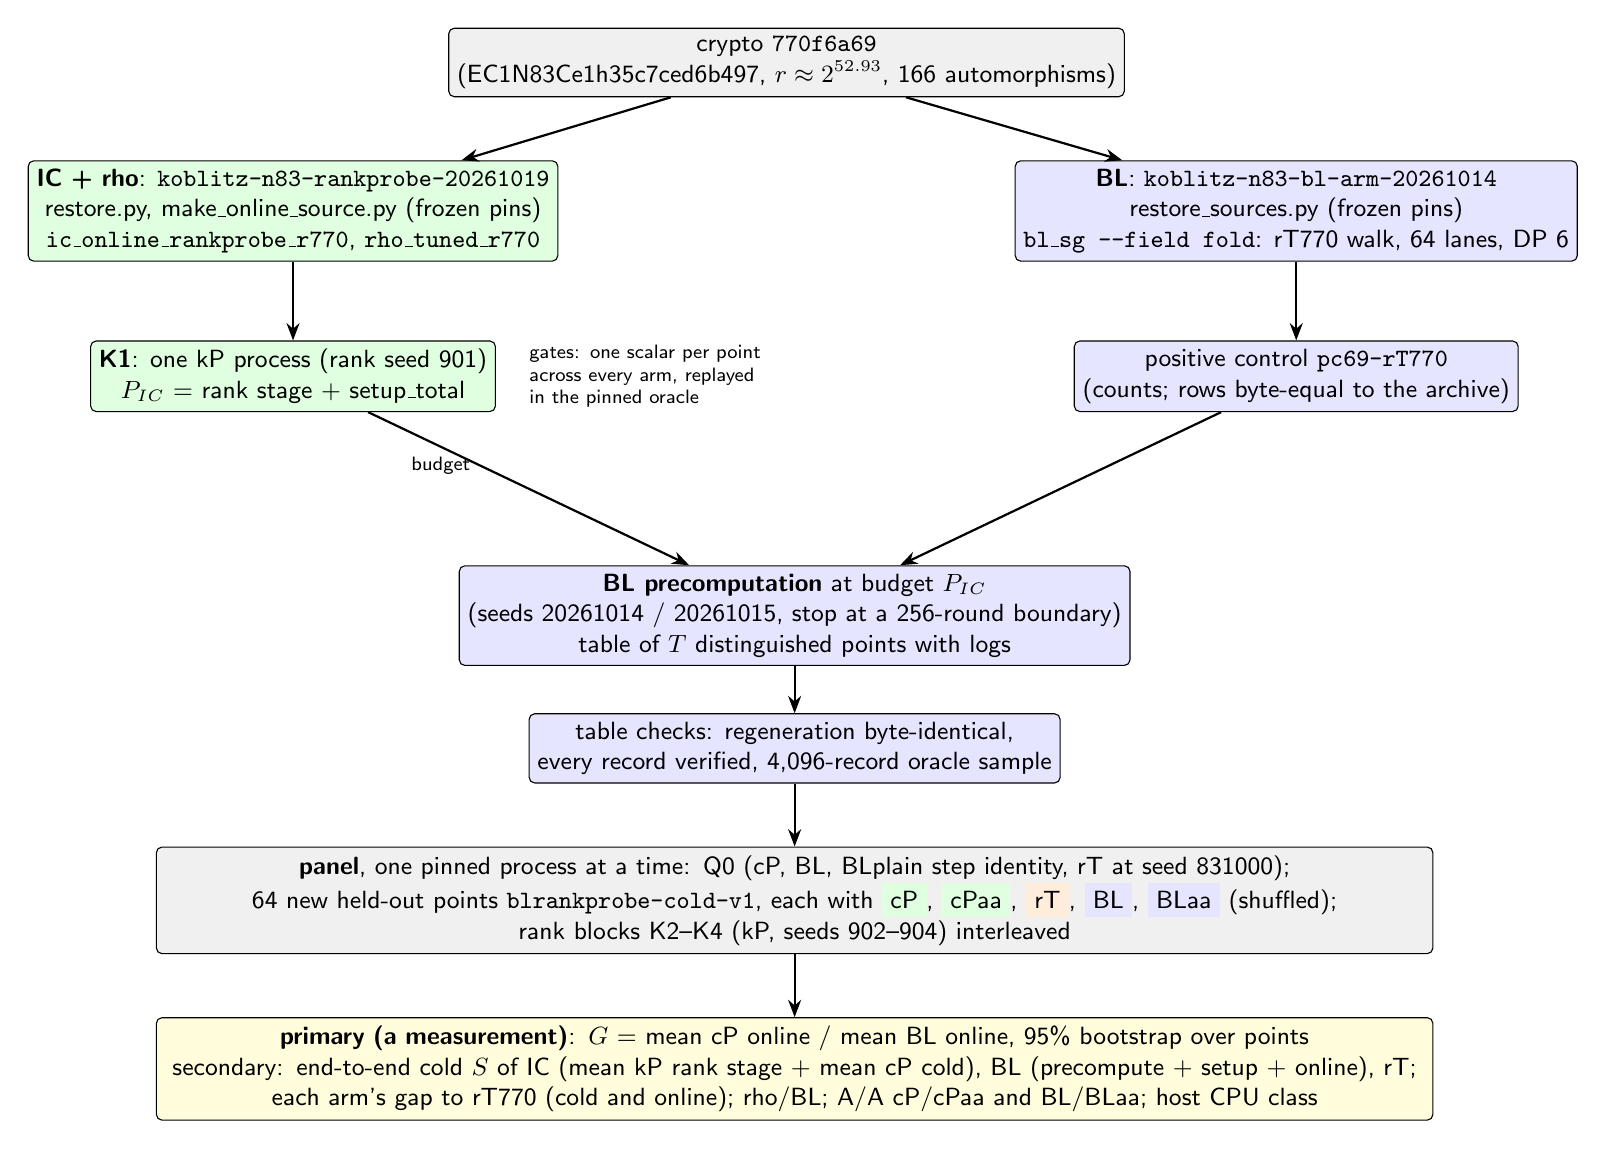
\begin{tikzpicture}[
  font=\sffamily\small,
  box/.style={draw, rounded corners=2pt, align=center, minimum height=8mm, inner sep=3pt},
  src/.style={box, fill=gray!12},
  ic/.style={box, fill=green!12},
  bl/.style={box, fill=blue!10},
  rho/.style={box, fill=orange!14},
  res/.style={box, fill=yellow!14},
  arr/.style={-{Stealth[length=2.2mm]}, thick},
  note/.style={align=left, font=\sffamily\scriptsize}
]
\node[src] (crypto) {crypto \texttt{770f6a69}\\(EC1N83Ce1h35c7ced6b497, $r\approx 2^{52.93}$, 166 automorphisms)};
\node[ic, below left=8mm and -14mm of crypto] (icsrc) {\textbf{IC + rho}: \texttt{koblitz-n83-rankprobe-20261019}\\restore.py, make\_online\_source.py (frozen pins)\\\texttt{ic\_online\_rankprobe\_r770}, \texttt{rho\_tuned\_r770}};
\node[bl, below right=8mm and -14mm of crypto] (blsrc) {\textbf{BL}: \texttt{koblitz-n83-bl-arm-20261014}\\restore\_sources.py (frozen pins)\\\texttt{bl\_sg -{}-field fold}: rT770 walk, 64 lanes, DP 6};
\draw[arr] (crypto) -- (icsrc); \draw[arr] (crypto) -- (blsrc);

\node[ic, below=10mm of icsrc] (k1) {\textbf{K1}: one kP process (rank seed 901)\\$P_{IC}$ = rank stage + setup\_total};
\node[bl, below=10mm of blsrc] (ctl) {positive control \texttt{pc69-rT770}\\(counts; rows byte-equal to the archive)};
\node[bl, below=24mm of $(k1)!0.5!(ctl)$] (pre) {\textbf{BL precomputation} at budget $P_{IC}$\\(seeds 20261014 / 20261015, stop at a 256-round boundary)\\table of $T$ distinguished points with logs};
\node[bl, below=6mm of pre] (chk) {table checks: regeneration byte-identical,\\every record verified, 4,096-record oracle sample};
\draw[arr] (icsrc) -- (k1); \draw[arr] (blsrc) -- (ctl);
\draw[arr] (k1) -- node[note, left, pos=0.35] {budget} (pre); \draw[arr] (ctl) -- (pre);
\draw[arr] (pre) -- (chk);

\node[src, below=8mm of chk, text width=160mm] (panel) {\textbf{panel}, one pinned process at a time: Q0 (cP, BL, BLplain step identity, rT at seed 831000);\\
64 new held-out points \texttt{blrankprobe-cold-v1}, each with \colorbox{green!12}{cP}, \colorbox{green!12}{cPaa}, \colorbox{orange!14}{rT}, \colorbox{blue!10}{BL}, \colorbox{blue!10}{BLaa} (shuffled);\\
rank blocks K2--K4 (kP, seeds 902--904) interleaved};
\draw[arr] (chk) -- (panel);

\node[res, below=8mm of panel, text width=160mm] (res) {\textbf{primary (a measurement)}: $G$ = mean cP online / mean BL online, 95\% bootstrap over points\\
secondary: end-to-end cold $S$ of IC (mean kP rank stage + mean cP cold), BL (precompute + setup + online), rT;\\
each arm's gap to rT770 (cold and online); rho/BL; A/A cP/cPaa and BL/BLaa; host CPU class};
\draw[arr] (panel) -- (res);
\node[note, right=3mm of k1, text width=30mm] {gates: one scalar per point\\across every arm, replayed\\in the pinned oracle};
\end{tikzpicture}
\end{document}
